\chapter{Architecture}
\label{chap:architecture}

%TODO
TODO: rework everything when you are done with the related work chapter.
See implementation stuff on garbage collection for deleted events, handling of conflicts, etc.

The following section will define the data model each peer keeps of its data and specify the API for updating it between peers.
First we will define and explain the model each peer keeps of the stored data.
Next the messages used to facilitate the update of the model between clients will be discussed.
Finally we will take a look at the advanced features and how they will be built on top of the previous work.

\section{Peer Data Model}

%TODO: ignore files / dirs? This should be implemented...

% why again json
Since we intend to use JSON for communication via Tox, it seems prudent to define the file model of a peer's data in the same way.
This will allow easy application of updates without having to explicitly translate between two different views of the same data.

An important feature that the model must have is that it works independent of the file types.
Therefore there are only two assumptions we will make of the structure of the directory that a peer will work on: namely that it contains files sorted in directories.
Out of this we can immediately synthesize our two main components we will require: a file model and a directory model.
Since a peer is intended to have directory as the root node from which to run, the core element will always be a directory.
An example of the proposed model structure can be seen in~\ref{list:model}.

\begin{figure}[htp]
\begin{modellist}
\item Root Directory
    \begin{modellist}
        \item File
        \item Sub Directory
            \begin{modellist}
                \item File
                \item File
            \end{modellist}
        \item File
        \item File
    \end{modellist}
\end{modellist}
\caption[Data Model Example Structure]{An example of how a data model of a directory is structured.}
\label{list:model}
\end{figure}

The most important aspect is of course what information is stored within the model and its objects.
Each file is considered a binary blob and not modified by Tinzenite in any way to preserve data integrity.
Therefore additional information that Tinzenite requires to function will need to be part of the model.

Each object in the model will for identification purposes be specified by a hash.
This hash will be a unique randomly generated hash.
This hash allows us to decouple the name of the object from its model representation, effectively serving the same function as node identification numbers when stored on a disk.
This is required so that we can differentiate a renamed file from a removed file and update a model accordingly.
Furthermore each model object will contain a path variable that specifies the complete path of the object in the directory tree.
This has the purpose of allowing the placement of all files in the correct locations on disk.
Notably, unlike on the user's disk, the names contained in the path are the identifying hashes.

Apart from the above attributes Tinzenite must also track versions of files to allow detection of when files have been updated.
We will use a vector clock\footnote{TODO: find and link paper?} to implement this.
The vector of peers with the associated versions can also be used to detect collisions.
Some further attributes will also be specified, but as they differ between file and directory model, these will be further discussed in the corresponding sections below.

It is important to note that the model will not be used to store peer reliant information.
This includes for example where the directory is placed on the peer's file system.
Such information must be stored separately by the peer and applied when working with the data model, for example when determining what the full path on the file system will be for a file that is to be written.
Some properties are also not suited to be transferred between peers.
This includes file system or operating system dependent properties such as usage rights, ownership, or flags.
%TODO look into this. A security argument might be to simply strip all extra information on transit but leave it untouched on client side, even over file updates. This would mean that the user only has to setup a dir once with rights etc as he likes it before he can use it with Tinzenite.

\subsection{Directory Model}
\label{sec:dir_model}

\begin{figure}[htp]
    \begin{lstlisting}[language=json,firstnumber=0]
    {
        "identification":"subdir_random_hash",
        "path":"root_hash/subdir_random_hash",
        "name":"subdir",
        "version":{
            "peer_name", "version",
            "peer_name", "version",
            ...
        },
        "objects":[
            ...
        ]
    }
    \end{lstlisting}
\caption[Directory JSON Model]{An example of a directory JSON object. Note that for brevity no files or sub directories are shown in the \textit{"objects"} array.}
\label{json:directory_model}
\end{figure}

Figure~\ref{json:directory_model} shows an example of the proposed JSON structure for representing a directory.
The \textit{"identification"} attribute is a random generated hash that uniquely identifies the directory.
The \textit{"path"} attribute stores the concatenated relative full path from the peers root directory, notably replacing the real names of the directories with the corresponding identification attribute values.
For trusted peers that store an unencrypted version of the directory the clear text \textit{"name"} is also stored here as an attribute.
To differentiate between updates we require a \textit{"version"} attribute which represents a vector clock of peers and their last known version.
Finally an \textit{"objects"} array is where the corresponding sub directories or files are placed.

\subsection{File Model}
\label{sec:file_model}

\begin{figure}[htp]
    \begin{lstlisting}[language=json,firstnumber=0]
    {
        "identification":"file_random_hash",
        "path":"root_hash/subdir_random_hash/file_random_hash",
        "name":"file",
        "version":{
            "peer_name", "version",
            "peer_name", "version",
            ...
        },
        "content":"content_hash",
        "shadow":"false"
    }
    \end{lstlisting}
\caption[File JSON Model]{An example of a file JSON object.}
\label{json:file_model}
\end{figure}

Figure~\ref{json:file_model} shows an example of the proposed JSON structure for representing a file object.
The \textit{"identification"} attribute is a random generated hash that uniquely identifies the file.
The \textit{"path"} attribute stores the concatenated relative full path from the peers root directory, notably replacing the real names of the directories with the corresponding identification hashes, and finally the file name with its hash too.
For trusted peers that store an unencrypted version of the file the clear text \textit{"name"} is also stored here as an attribute.
To differentiate between updates we require a \textit{"version"} attribute which represents a vector clock of peers and their last known version.
Important for detecting file changes is the \textit{"content"} attribute which stores a hash of the file's binary blob.
Finally the \textit{"shadow"} flag is used to notify a peer whether the file is locally accessible or must first be fetched from other peers.

\subsection{Peer Futher Data}

%TODO
TODO: the peer will contain more stuff than just the model (although ideally the model would encompass everything).
Need to also look at and introduce: deletion updates (can be model OR peer!) and peer list (how is this synced? needs to be considered!).

\begin{figure}[htp]
    \begin{lstlisting}[language=json,firstnumber=0]
    {
        "user":"hash_of_username.salt",
        "directory_id":"random_hash",
        "key":"encrypted_data.salt",
        "active_peers":[
            "peer_tox_id",
            ...
        ],
        "removed_peers":[
            "peer_tox_id",
            ...
        ]
    }
    \end{lstlisting}
\caption[Authentication JSON Object]{Shows the proposed contents of the authentication block. Apart from identifying information and the encrypted data encryption key note the peer lists – one for active peers and one for removed peers.}
\label{json:auth_object}
\end{figure}

Figure~\ref{json:auth_object} shows the management block that a peer keeps.
The value of \textit{"user"} allows the allocation of a directory to a user name.
This is important for example for the support of encrypted third party peers: they can attach accounts to the provided user name for controlling server side access.
Therefore we also need a way to distinguish multiple synchronized directories from each other: this is the random unique hash stored in \textit{"directory\_id"}.
Again, this can be used by third party service providers to differentiate the amount of directories that a user can store with them.
The symmetric key for encrypting and decrypting data for encrypted peers is stored in \textit{"key"}, encrypted in turn by a to be defined scheme that decrypts it upon entry of the correct password by the user.

Note that changing any of the values in the authentication block is not supported initially.
To change the password or the user name hash, the Tinzenite peer must be removed and added anew.
While cumbersome it offers the highest level of protection against possible security risks for now.

Finally we also use the authentication block to store and synchronize the peer list of connected peers of a synchronized directory.
As peers can be removed we need to keep a list of removed peers too.
Peers that have been removed, thus placing their Tox identification within the removed list, can not be reactivated.
The peer must be recreated and added as if it were a new peer.
Since we do not expect a large number of peers to be removed and added over the lifetime of a Tinzenite directory, this list is never trimmed.
A peer can detect a new peer by noticing its existence upon synchronization with another peer.
If the new peer Tox identification is not in the removed list it is simply added to the active list.
This ensures that peers that have been removed will never be added back to the active list which might pose a security risk\footnote{TODO: do something similar for removing files. Note that we WILL have to trim that list though at some point in time, but since we know which peers are active, this should be doable.}.

\section{Core Update API}

This section describes the API that will be used to synchronize two models on separate peers where the models might diverge.
To understand how this works, it is important to understand how Tinzenite is structured.

Every peer views all connected peers as separate connections.
A swarm behavior only comes to pass because of the independent actions of every peer, not through a combined communication between multiple peers.
This primarily makes it relatively easy to implement a Tinzenite peer, as the communication state is never between multiple peers.
Therefore a single peer has a base state of no connected other peers.

\subsection{Connection Management}
\label{sec:conn_management}

In this section we will discuss how Tinzenite connects to other peers.
As we distinguish between trusted and encrypted peers we must determine how the data we will send is to be modified accordingly.
If the initiating peer is already encrypted, the connection by default will be considered anonymous.
If not the peer must query the other peer.
Since we can not trust the other peer to give an honest answer this query must be cryptographically secure.
Attackers that illegitimately wants to connect to a trusted peer thus can not establish a clear connection without the required keys, which they should not be in possession of\footnote{Tinzenite is designed to avoid revealing keys to outsiders. However outside attacks are beyond its control such as for example key loggers.}.
Only if the challenge is successfully replied to is the other peer considered trusted and the following communication not anonymous.
If the challenge is ignored the other peer is considered as an encrypted peer and the following communication adapted to fit.
Should the challenge be incorrectly answered we can consider possibly warning the user or even blacklisting the peer.

Once the connection type has been determined it will be applied to all following communication.
In general this means that compared to a trusted communication identifying information and file contents will be encrypted.
The peer list will be synchronized but the encryption keys not.
The model exchange and all update messages will be partially encrypted too to preserve data security.

The next and final step to a ready and idle connection state is the exchange of models.
Once this is done both peers can compare the received models with their local ones and determine which files they need to update from the other peer.
These messages will then be sent asynchronously over the now established and typified communication channel accordingly.

\begin{figure}[htp]
\centering
    \includegraphics[width=\textwidth]{graph/sm_peer_communications}
\caption[Connection State Diagram]{This diagram shows how peers handle the establishment of a connection to a known peer.}
\label{graph:connection_states}
\end{figure}

Figure~\ref{graph:connection_states} shows an informal state diagram of how a peer reaches the idle state where the connection is ready and set up.
The switch from the disconnected state to the connected state is signaled by the underlying Tox connection, meaning it happens when the other peer is online and visible via the Tox channel.
Once connected and if the peer itself is a trusted peer, a challenge is sent which contains a general identifier and an encrypted nonce.
The encrypted nonce is important to check whether the other peer is encrypted or trusted.

Note that a few points must be considered that can not be shown in the diagram.
Since Tinzenite is designed as a peer to peer network, no client server structure exists.
This poses the challenge of who begins the construction of a connection, especially as we can not distinguish between peers that have been online for a while already and peers that just activated when the base peer starts up.
This is due to peer to peer architecture of Tox: not all peers will respond to queries within the same time frame.
Peers further away from a network perspective will seem to be online only after peers that are nearer.
We solve this issue by having the peers use a random back off time whenever a request expects an answer\footnote{For example the challenge message for establishing a trusted connection.}.

Since we can not trust the other side of the Tox channel to be a Tinzenite peer, the peer initiating a connection will not advance beyond a step where it expects an answer.
This means that for example an attacker would either receive only a challenge (to which he can't respond without knowing the keys) or the anonymized model and peer list\footnote{The peer list is the more problematic of the two as it can be used to determine the size of the user's Tinzenite peer network. However to allow encrypted peers to facilitate file transfer between two mutually exclusively online peers, it must know this information. This is mitigated by the fact that Tox IDs are hard to guess and not shared beyond the Tinzenite peer network. TODO: move this to the security section / chapter / whatever?} (which doesn't offer up any useful information as per specifications).

\subsection{New Connection Establishment}

The previous section described how Tinzenite connects to known peers.
This section therefore discusses how Tinzenite connects to new peers, meaning peers that the user adds to the network.
Notably this is a manual process where the user is used as a secondary channel to prevent man in the middle attacks.
Since a typical Tinzenite network might have many peers, it is not desirable to have to authenticate a new peer manually with every other peer.
We therefore propose that the user only need authenticate the new peer with one existing peer.
From there the authentication is synchronized to the other existing peers much like any other file or property update.
This bootstrapping process allows a user friendly setup of peers.
Should the same peer have been added multiple times at different existing peers Tinzenite will detect this and merge the authentication together.

\begin{figure}[htp]
\centering
    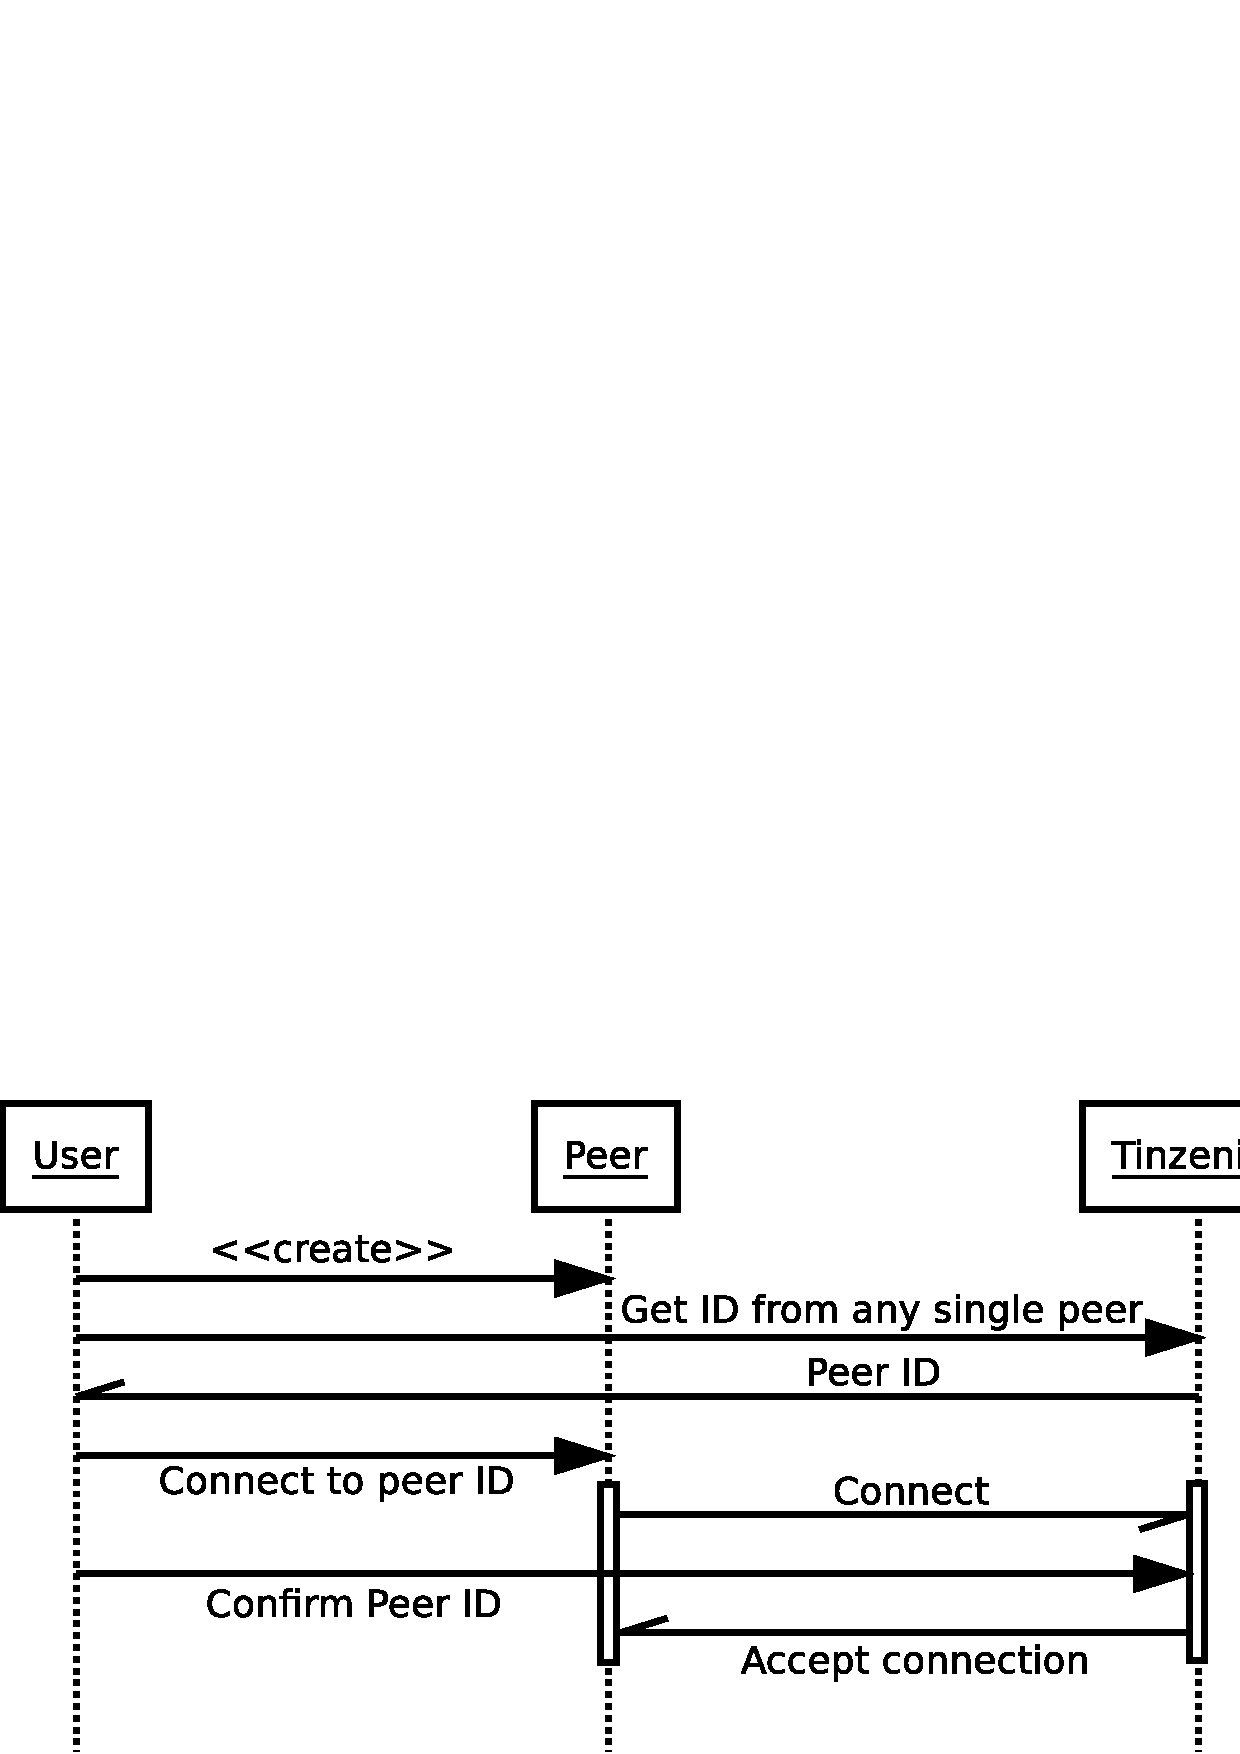
\includegraphics[width=10cm]{diagram/sequence_new_connect}
\caption[New Connection Sequence Diagram]{This diagram shows the interaction required to connect a new peer to the existing Tinzenite network.}
\label{diagram:new_connection}
\end{figure}

TODO: missing password entry that allows the new peer to become a trusted peer!
User must enter password that decrypts symmetric key.
Will need to think of a way to change the password if required... :P

Figure~\ref{diagram:new_connection} shows how a user interacts with a Tinzenite peer and the Tinzenite network (consisting of 1 to n other existing peers) to connect a new peer to the network for the first time.
As prose: the users simply start the new peer client for the first time.
Then they can point it at the directory location, change settings, and check that another peer is visible.
To establish an initial connection a Tox ID of an available trusted\footnote{Note that to set up a trusted peer the initial connection must also be to a trusted peer so that all encryption keys can be shared. If the available peer is only an encrypted one the new peer can also only be an encrypted peer as the keys for decrypting the files and data aren't available.} Tinzenite peer is required.
The users can then command the new peer to connect to this available peer by entering the Tox ID.
To ensure that no man in the middle attack can happen the users will now have to confirm the connection on the available peer.
This means allowing the connection there and ideally ensuring that the seen Tox ID is identical with the new peer's Tox ID.
Once the connection has been confirmed on the other peer a channel is opened.
The new peer address and its information will now be synchronized throughout the already connected peers once they are available, removing the need to add the new peer manually to each and every one.
The directories will immediately begin synchronization.

Removing peers will work much in the same way from a system perspective.
A user can note a peer to be removed, resulting in it being removed immediately from the peer where the action was initiated.
It will then transit through online peers and result in a complete removal once all peers have been online.
An interesting aspect to how to handle removal from the perspective of the to be removed peer is what to do with the data on the peer.
For a trusted peer we might offer a choice whether to remove the data or simply disconnect it from the Tinzenite network.
On the other hand encrypted peers can simply remove the data immediately as they can't access it anyway.

\subsection{Model Management}

This section will describe how a peer receives and sends messages via the Tox channel.
Since we will be required to distinguish between encrypted and trusted connections we will start off with the trusted one and then briefly highlight the differences required for an encrypted connection.

Once the setup has been completed, as seen in section~\ref{sec:conn_management}, the models must be updated if they do not match.
This happens normally when files and directories have changed through user or system interaction.

\subsubsection{Fetch File Message}

\begin{figure}[htp]
    \begin{lstlisting}[language=json,firstnumber=0]
    {
        "operation":"fetch",
        "identification":"object_identification_hash",
        "TODO":"ADD LIBRSYNC STUFF HERE",
        "delta":"true/false"
    }
    \end{lstlisting}
\caption[Fetch Object Message]{The message sent to initiate a file transfer.}
\label{json:fetch_file}
\end{figure}

Figure~\ref{json:fetch_file} shows how a message to initiate a file transfer is structured.
Note that apart from the identification we require no further information – the model has been independently updated.
Now the peers need only get the binary files.
Upon receiving the message the other peer starts a Tox file transfer which the initiating peer knows to accept as it just requested it.

TODO: add capability for delta updates... if possible. :P
Delta is difficult because we must effectively track parts of files instead of complete files... how to do this?
use librsync! <-- Really good and easy to use, will save a ton of work!

TODO: Also remember that multiple file transfers might be a problem.
Do we limit the connection to one transfer at a time or can we fetch everything at once?

\subsubsection{Update Object Message}

\begin{figure}[htp]
    \begin{lstlisting}[language=json,firstnumber=0]
    {
        "operation":"create",
        "object":{
            ...
        }
    }
    \end{lstlisting}
\caption[Update Object Message]{The message broadcast by a peer to connected peers to notify that an update has happened.}
\label{json:update_object}
\end{figure}

Figure~\ref{json:update_object} is a message for broadcasting a model update to other connected peers.
The update message serves to keep both models in sync even after the initial synchronization at connection establishment.
Upon receiving an update message the peer will most likely immediately respond with a fetch message to retrieve the updated file.

What happens within a peer's model upon receiving such an update message differs on what kind of file operation it is.
There exist just four cases from Tinzenite's view: either the content has changed, a file attribute has changed, a file has been created, or a file has been removed.

%TODO refer forwards to Tinzenite logic once I've worked that out
Tinzenite continously checks the directory against the model of the same (see also TODO).
In the case that it notices that a file is missing from the directory but that exists in the model Tinzenite fetches and creates that file.

TODO: autsch, how to handle file deletions?
They must be caught and handled correctly!
I must synchronize and keep tab on which files have once existed and have been since deleted... :(

In the case that the content has changed the \textit{"content"} attribute must be updated and a fetch message sent to retrieve the binary file so that the model matches the directory again.
Somewhat more interesting is the case where the content remains the same

What doesn't change from the system view is the contents of the file, which in turn means that the content hash remains the same, and its identification hash.
Within the file model (compare section~\ref{sec:file_model}) this translates to changes to the \textit{"path"}, \textit{"name"}, and \textit{"version"} attributes.

%TODO
TODO: how are conflicts handled.
Easiest: clients detect files are same but different, create the two as new versions and rename so user can see.
Nothing else needs to change for the API then – if the user resolves it manually the rename / delete of files will propagate as normal.

TODO: on receiving an update: queue in connection specific command queue (one per connection because only one OP per connection) (update / redo existing fetch if applicable != FIFO); fetch first file in queue.
Then wait a bit (?) before propagating update yourself (decouple receive and send time frames?). <-- Isn't this implementation details?

\section{Advanced Features API}

TODO: Here is the list of what I consider to be the advanced features.
Now do something sensible with it.

\begin{description}[leftmargin=2em,style=nextline,noitemsep,nolistsep]
\item[Encryption Key Management]
    An important capability will be the synchronization of the access keys to unencrypted clients so that all of them can access the data stored on encrypted clients.
    Thoughts should be given to how to revoke compromised keys.
\item[Space Management]
    The API must respect differences in storage size capabilities between different clients or size restrictions.
    Notably this is important for third parties to sell different storage sizes to clients.
    TODO: could files above the limit be sent as shadow files?
\item[Shadow Files]
    Depending on the location of a client a user may with to only access specific files without having to get an entire set or updates.
    Therefore the client could be set to only read and create dummy files.
    By selecting specific files the client will then only update or retrieve the corresponding files or directories.
    TODO: what to do if a client knows of shadow files but can't get full set?
    Are shadow files also transitively synchronized?
\end{description}
